\section{Introduction}\label{introduction-000}

The HVAC-Diagram program is a simple utility that can be used to generate a svg file based on the bnd file generated by EnergyPlus. It is a stored in the primary EnergyPlus\textbackslash{}PostProcessor folder upon installation.

It creates a series of diagrams for the layout of the HVAC system components. The SVG file can be viewed with a number of internet browser plug-ins such as produced by Adobe that can be downloaded at \href{http://www.adobe.com/svg}{www.adobe.com/svg}. To get help within the Adobe viewer, right click anywhere on the drawing.

Each diagram should be read from left to right, which is the direction of the flow of the fluid through the components.

The HVAC-Diagram program is automatically called when using EP-Launch but can also be included in other batch files. To view the drawing in EP-Launch, click on the drawing button. You can zoom in on this drawing and with the ``copy'' command, paste a zoomed in portion as a bitmap in your document.

\begin{figure}[hbtp] % fig 32
\centering
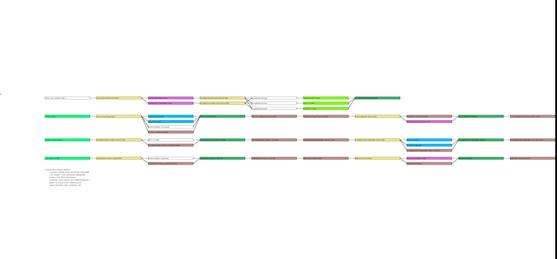
\includegraphics[width=0.9\textwidth, height=0.9\textheight, keepaspectratio=true]{media/image030.jpg}
\caption{HVAC Diagram -- SVG Drawing \protect \label{fig:hvac-diagram-svg-drawing}}
\end{figure}

Objects that are recognized by the HVAC diagram are shown in Table~\ref{table:hvac-diagram-object-names-primary-sort-colors} (sorted by Object Name) and Table~\ref{table:hvac-diagram-object-names-and-color-primary} (sorted by color).

% table 30
\begin{longtable}[c]{@{}ll@{}}
\caption{HVAC Diagram Object Names (primary sort) Colors \label{table:hvac-diagram-object-names-primary-sort-colors}} \tabularnewline
\toprule 
Object Name & Color \tabularnewline
\midrule
\endfirsthead

\caption[]{HVAC Diagram Object Names (primary sort) Colors} \tabularnewline
\toprule 
Object Name & Color \tabularnewline
\midrule
\endhead

AirLoopHVAC:ReturnPlenum & lightgreen \tabularnewline
AirLoopHVAC:SupplyPlenum & lightgreen \tabularnewline
AirLoopHVAC:ZoneMixer & wheat \tabularnewline
AirLoopHVAC:ZoneSplitter & wheat \tabularnewline
AirTerminal:DualDuct:ConstantVolume & wheat \tabularnewline
AirTerminal:DualDuct:VAV & wheat \tabularnewline
AirTerminal:SingleDuct:Uncontrolled & none \tabularnewline
AirTerminal:SingleDuct:VAV:NoReheat & wheat \tabularnewline
AirTerminal:SingleDuct:VAV:Reheat & wheat \tabularnewline
Boiler:HotWater & indianred \tabularnewline
Chiller:Absorption & powderblue \tabularnewline
Chiller:CombustionTurbine & powderblue \tabularnewline
Chiller:ConstantCOP & powderblue \tabularnewline
Chiller:Electric & powderblue \tabularnewline
Chiller:EngineDriven & powderblue \tabularnewline
ChillerHeater:Absorption:DirectFired & powderblue \tabularnewline
Coil:Cooling:DX:MultiSpeed & skyblue \tabularnewline
Coil:Cooling:DX:SingleSpeed & skyblue \tabularnewline
Coil:Cooling:Water & skyblue \tabularnewline
Coil:Cooling:Water:DetailedGeometry & skyblue \tabularnewline
Coil:Cooling:WaterToAirHeatPump:EquationFit & skyblue \tabularnewline
Coil:Cooling:WaterToAirHeatPump:ParameterEstimation & skyblue \tabularnewline
Coil:Heating:DX:SingleSpeed & skyblue \tabularnewline
Coil:Heating:Electric & salmon \tabularnewline
Coil:Heating:Gas & salmon \tabularnewline
Coil:Heating:Water & salmon \tabularnewline
Coil:Heating:WaterToAirHeatPump:EquationFit & salmon \tabularnewline
Coil:Heating:WaterToAirHeatPump:ParameterEstimation & salmon \tabularnewline
Connector:Mixer & lightgreen \tabularnewline
Connector:Splitter & wheat \tabularnewline
Controller:OutdoorAir & none \tabularnewline
Controller:WaterCoil & none \tabularnewline
CoolingTower:SingleSpeed & pink \tabularnewline
Dehumidifier:Desiccant:NoFans & tan \tabularnewline
DistrictCooling & none \tabularnewline
DistrictHeating & none \tabularnewline
EvaporativeCooler:Direct:CelDekPad & aliceblue \tabularnewline
EvaporativeCooler:Indirect:CelDekPad & aliceblue \tabularnewline
EvaporativeCooler:Indirect:ResearchSpecial & aliceblue \tabularnewline
Fan:ConstantVolume & silver \tabularnewline
Fan:OnOff & silver \tabularnewline
Fan:VariableVolume & silver \tabularnewline
Fan:ZoneExhaust & silver \tabularnewline
Generator:CombustionTurbine & orange \tabularnewline
Generator:InternalCombustionEngine & orange \tabularnewline
GroundHeatExchanger:Pond & paleturquoise \tabularnewline
GroundHeatExchanger:Surface & paleturquoise \tabularnewline
GroundHeatExchanger:Vertical & paleturquoise \tabularnewline
HeatExchanger:AirToAir:FlatPlate & paleturquoise \tabularnewline
HeatExchanger:AirToAir:SensibleAndLatent & paleturquoise \tabularnewline
HeatExchanger:Hydronic & paleturquoise \tabularnewline
HeatPump:WaterToWater:EquationFit:Cooling & lightslategray \tabularnewline
HeatPump:WaterToWater:EquationFit:Heating & lightslategray \tabularnewline
HeatPump:WaterToWater:ParameterEstimation:Cooling & lightslategray \tabularnewline
HeatPump:WaterToWater:ParameterEstimation:Heating & lightslategray \tabularnewline
Humidifier:Steam:Electric & lavender \tabularnewline
LoadProfile:Plant & none \tabularnewline
OutdoorAir:Mixer & lawngreen \tabularnewline
OutdoorAir:NodeList & none \tabularnewline
Pipe:Adiabatic & wheat \tabularnewline
PlantLoopConnection & wheat \tabularnewline
Pump:ConstantSpeed & springgreen \tabularnewline
Pump:VariableSpeed & springgreen \tabularnewline
SolarCollector:FlatPlate:Water & yellow \tabularnewline
WaterHeater:Mixed & orange \tabularnewline
WaterHeater:Stratified & orange \tabularnewline
ZoneHVAC:Baseboard:Convective:Water & salmon \tabularnewline
ZoneHVAC:EnergyRecoveryVentilator:Controller & none \tabularnewline
ZoneHVAC:EquipmentConnections & chartreuse \tabularnewline
ZoneHVAC:IdealLoadsAirSystem & none \tabularnewline
ZoneHVAC:LowTemperatureRadiant:ConstantFlow & orangered \tabularnewline
ZoneHVAC:LowTemperatureRadiant:VariableFlow & orangered \tabularnewline
ZoneHVAC:UnitVentilator & sandybrown \tabularnewline
\bottomrule
\end{longtable}

% table 31
\begin{longtable}[c]{@{}ll@{}}
\caption{HVAC Diagram Object Names and Color (primary sort) \label{table:hvac-diagram-object-names-and-color-primary}} \tabularnewline
\toprule 
Object Name & Color \tabularnewline
\midrule
\endfirsthead

\caption[]{HVAC Diagram Object Names and Color (primary sort)} \tabularnewline
\toprule 
Object Name & Color \tabularnewline
\midrule
\endhead

EvaporativeCooler:Direct:CelDekPad & aliceblue \tabularnewline
EvaporativeCooler:Indirect:CelDekPad & aliceblue \tabularnewline
EvaporativeCooler:Indirect:ResearchSpecial & aliceblue \tabularnewline
ZoneHVAC:EquipmentConnections & chartreuse \tabularnewline
Boiler:HotWater & indianred \tabularnewline
Humidifier:Steam:Electric & lavender \tabularnewline
OutdoorAir:Mixer & lawngreen \tabularnewline
AirLoopHVAC:ReturnPlenum & lightgreen \tabularnewline
AirLoopHVAC:SupplyPlenum & lightgreen \tabularnewline
Connector:Mixer & lightgreen \tabularnewline
HeatPump:WaterToWater:EquationFit:Cooling & lightslategray \tabularnewline
HeatPump:WaterToWater:EquationFit:Heating & lightslategray \tabularnewline
HeatPump:WaterToWater:ParameterEstimation:Cooling & lightslategray \tabularnewline
HeatPump:WaterToWater:ParameterEstimation:Heating & lightslategray \tabularnewline
AirTerminal:SingleDuct:Uncontrolled & none \tabularnewline
Controller:OutdoorAir & none \tabularnewline
Controller:WaterCoil & none \tabularnewline
DistrictCooling & none \tabularnewline
DistrictHeating & none \tabularnewline
LoadProfile:Plant & none \tabularnewline
OutdoorAir:NodeList & none \tabularnewline
ZoneHVAC:EnergyRecoveryVentilator:Controller & none \tabularnewline
ZoneHVAC:IdealLoadsAirSystem & none \tabularnewline
Generator:CombustionTurbine & orange \tabularnewline
Generator:InternalCombustionEngine & orange \tabularnewline
WaterHeater:Mixed & orange \tabularnewline
WaterHeater:Stratified & orange \tabularnewline
ZoneHVAC:LowTemperatureRadiant:ConstantFlow & orangered \tabularnewline
ZoneHVAC:LowTemperatureRadiant:VariableFlow & orangered \tabularnewline
GroundHeatExchanger:Pond & paleturquoise \tabularnewline
GroundHeatExchanger:Surface & paleturquoise \tabularnewline
GroundHeatExchanger:Vertical & paleturquoise \tabularnewline
HeatExchanger:AirToAir:FlatPlate & paleturquoise \tabularnewline
HeatExchanger:AirToAir:SensibleAndLatent & paleturquoise \tabularnewline
HeatExchanger:Hydronic & paleturquoise \tabularnewline
CoolingTower:SingleSpeed & pink \tabularnewline
Chiller:Absorption & powderblue \tabularnewline
Chiller:CombustionTurbine & powderblue \tabularnewline
Chiller:ConstantCOP & powderblue \tabularnewline
Chiller:Electric & powderblue \tabularnewline
Chiller:EngineDriven & powderblue \tabularnewline
ChillerHeater:Absorption:DirectFired & powderblue \tabularnewline
Coil:Heating:Electric & salmon \tabularnewline
Coil:Heating:Gas & salmon \tabularnewline
Coil:Heating:Water & salmon \tabularnewline
Coil:Heating:WaterToAirHeatPump:EquationFit & salmon \tabularnewline
Coil:Heating:WaterToAirHeatPump:ParameterEstimation & salmon \tabularnewline
ZoneHVAC:Baseboard:Convective:Water & salmon \tabularnewline
ZoneHVAC:UnitVentilator & sandybrown \tabularnewline
Fan:ConstantVolume & silver \tabularnewline
Fan:OnOff & silver \tabularnewline
Fan:VariableVolume & silver \tabularnewline
Fan:ZoneExhaust & silver \tabularnewline
Coil:Cooling:DX:MultiSpeed & skyblue \tabularnewline
Coil:Cooling:DX:SingleSpeed & skyblue \tabularnewline
Coil:Cooling:Water & skyblue \tabularnewline
Coil:Cooling:Water:DetailedGeometry & skyblue \tabularnewline
Coil:Cooling:WaterToAirHeatPump:EquationFit & skyblue \tabularnewline
Coil:Cooling:WaterToAirHeatPump:ParameterEstimation & skyblue \tabularnewline
Coil:Heating:DX:SingleSpeed & skyblue \tabularnewline
Pump:ConstantSpeed & springgreen \tabularnewline
Pump:VariableSpeed & springgreen \tabularnewline
Dehumidifier:Desiccant:NoFans & tan \tabularnewline
AirLoopHVAC:ZoneMixer & wheat \tabularnewline
AirLoopHVAC:ZoneSplitter & wheat \tabularnewline
AirTerminal:DualDuct:ConstantVolume & wheat \tabularnewline
AirTerminal:DualDuct:VAV & wheat \tabularnewline
AirTerminal:SingleDuct:VAV:NoReheat & wheat \tabularnewline
AirTerminal:SingleDuct:VAV:Reheat & wheat \tabularnewline
Connector:Splitter & wheat \tabularnewline
Pipe:Adiabatic & wheat \tabularnewline
PlantLoopConnection & wheat \tabularnewline
SolarCollector:FlatPlate:Water & yellow \tabularnewline
\bottomrule
\end{longtable}
